\section{Architecture}

The architecture used on this project is the integration of three systems: Robot Shop \cite{robotshop}, ELK \cite{elk}, and MLog \cite{mlog}.

\begin{figure}[htbp]
\centering
\centerline{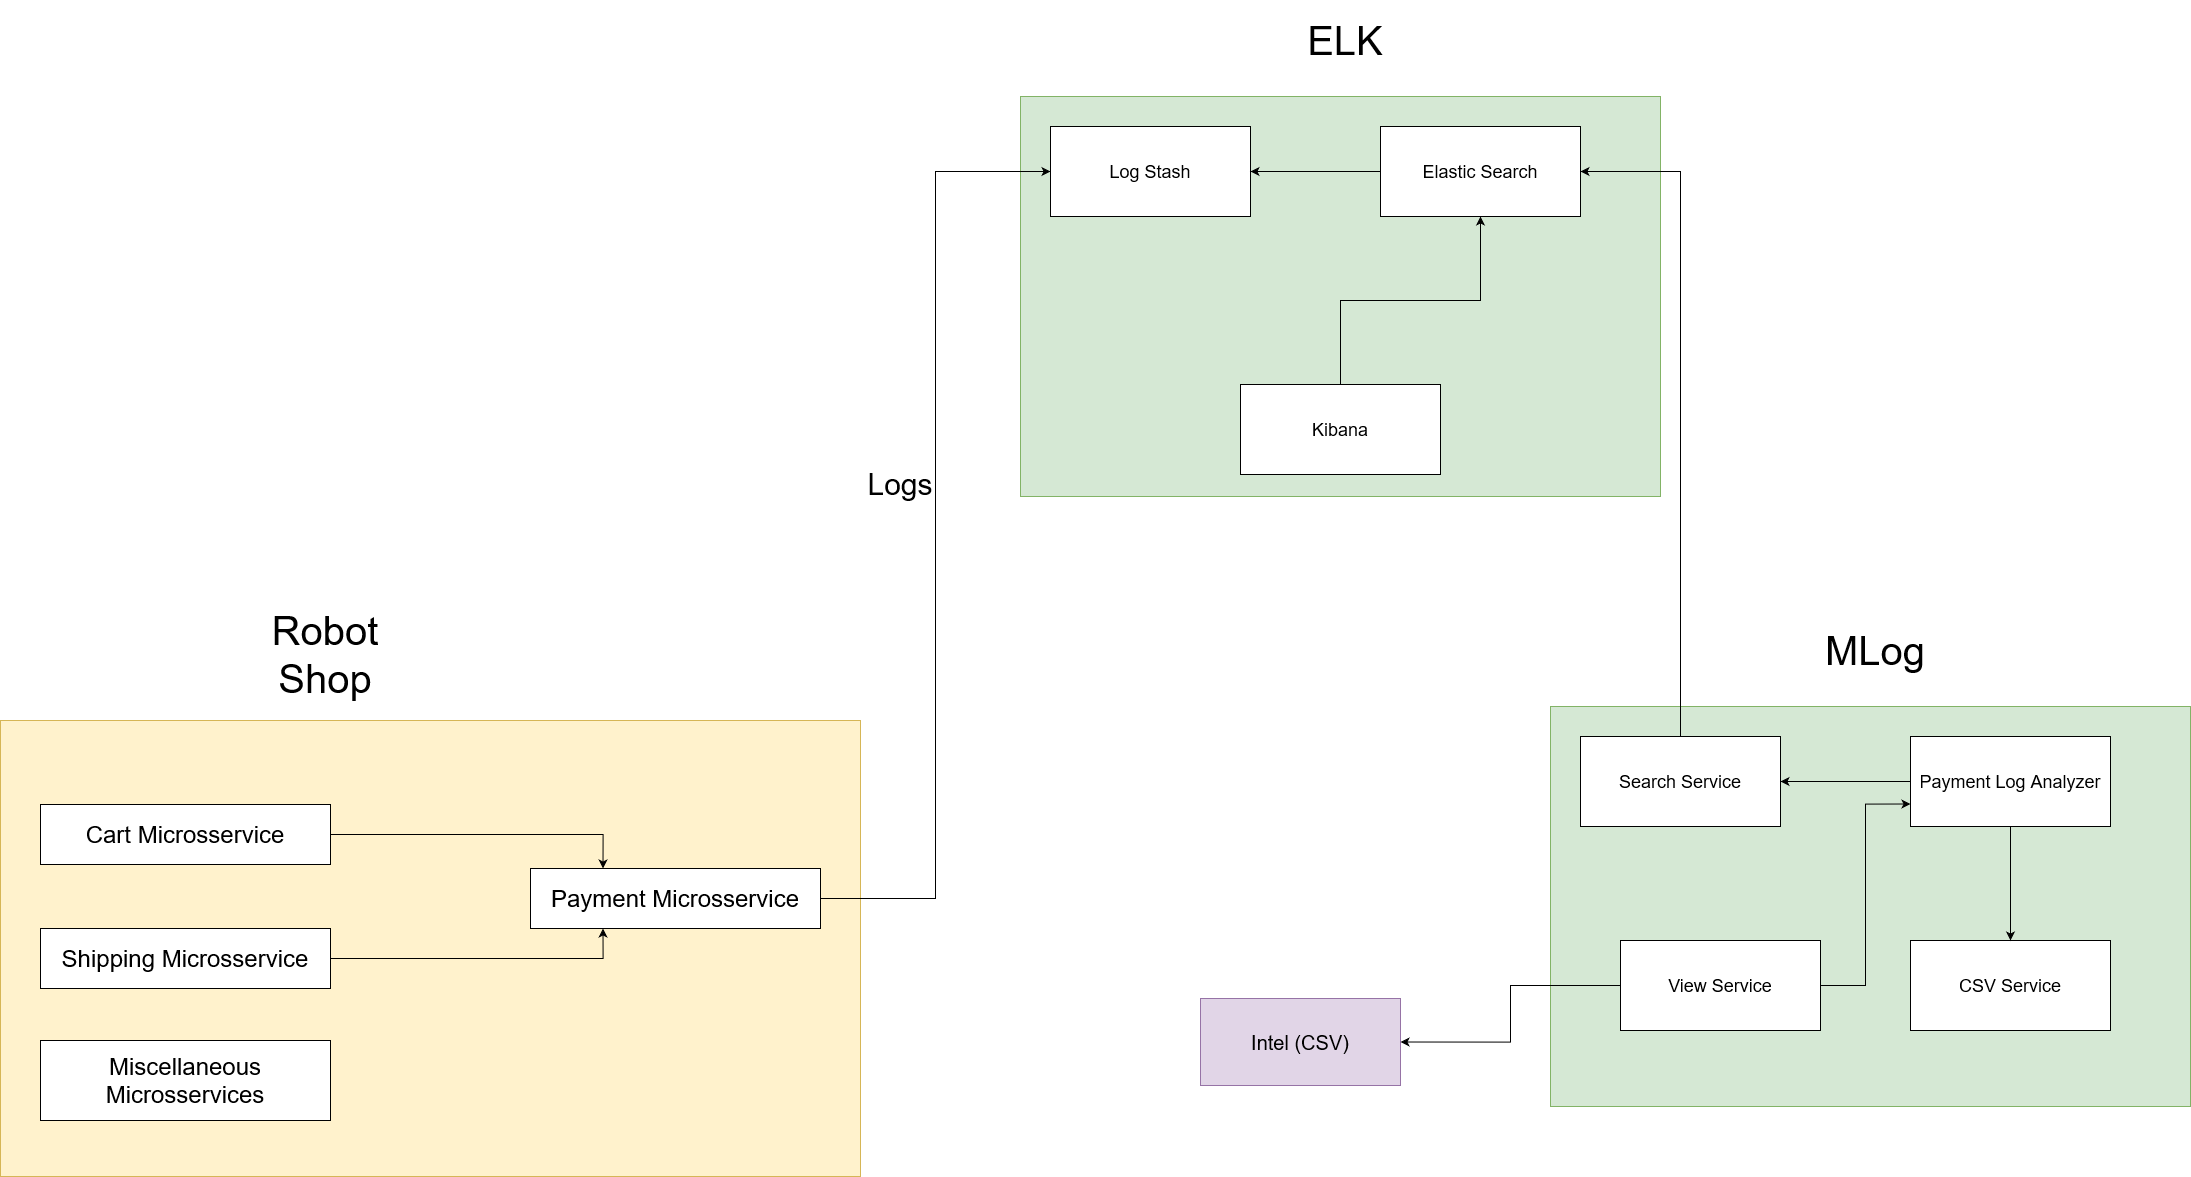
\includegraphics[width=0.5\textwidth]{Media/architecture.png}}
\caption{A generalized view of this project is architecture.}
\label{fig:architecture}
\end{figure}

\subsection{Robot Shop}

The e-commerce which logs were analyzed on this paper is the Robot Shop \cite{robotshop}, it is a simple microservices-based e-commerce with open source. There are 12 services on the Robot Shop, but the information analyzed is contained on the payment microservice, as this service carries the data of both shipping and cart services.

\begin{figure}[htbp]
\centering
\centerline{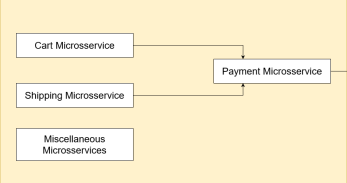
\includegraphics[width=0.5\textwidth]{Media/robot_shop.png}}
\caption{The Robot Shop is architecture}
\label{fig:architecture-robot-shop}
\end{figure}

\subsection{ELK}

ELK \cite{elk} is a project that groups Kibana \cite{kibana}, Elasticsearch \cite{elasticsearch} and Logstash \cite{logstash}. The logs generated on the payment microservice are sent and stored on Logstash. After creating an index pattern on Kibana, it is possible to see the logs store through kibana is interface. The Elasticsearch service is responsible for searching through the stored logs to analyze the data contained on the payment is logs.

\begin{figure}[htbp]
\centering
\centerline{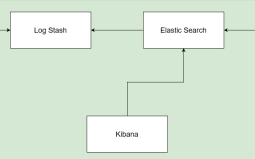
\includegraphics[width=0.5\textwidth]{Media/elk.png}}
\caption{The ELK is architecture}
\label{fig:architecture-elk}
\end{figure}

\subsection{MLog}

MLog \cite{mlog} is the project developed with this paper, and it consists on 4 microservices:

\begin{itemize}
  \item The view service, which is the front-end of MLog, it enables the filter and download of the analysis.
  \item The payment log analyzer service is the service that gets the processed data to find valuable information. It receives the request from the view service, then requests the processed data from the search service, and, after finding the information, it requests the download of the CSV with the intel found.
  \item Search service is the service that requests the queries to elastic search, it also processes the data further in order to get only the data about the purchase.
  \item CSV service is a common service that generates a CSV file based on the data present on the request.
\end{itemize}

\begin{figure}[htbp]
\centering
\centerline{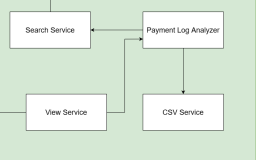
\includegraphics[width=0.5\textwidth]{Media/mlog.png}}
\caption{The MLog is architecture}
\label{fig:architecture-mlog}
\end{figure}